\chapter{Криволинейные, контурные и поверхностные интегралы}\label{chap:line-surface-integrals}\markright{Глава 35}

\section{Параметризованная кривая и два вида интеграла}
\begin{definition}\term{Параметризованная кривая} (\emph{parametrized curve}) задаётся \(\gamma(t)\in\mathbb R^n\), \(a\le t\le b\). Будем брать кусочно \(C^1\)-кривые с конечным числом гладких частей и ненулевой скоростью внутри каждой части. \par\term{Ориентация кривой} (\emph{orientation}) — выбранное направление прохождения от начала к концу.\end{definition}
\begin{definition}\term{Криволинейный интеграл первого рода} (\emph{scalar line integral}) непрерывной \(f\) равен
\[
\int_\gamma f\,ds=\int_a^b f(\gamma(t))\|\gamma'(t)\|\,dt.
\]
При \(f=1\) это длина кривой; при линейной плотности — масса проволоки.
\end{definition}
\begin{definition}\term{Криволинейный интеграл второго рода} (\emph{vector line integral; work integral}) непрерывного векторного поля равен
\[
\int_\gamma F\cdot d\symbf r
=\int_a^b\langle F(\gamma(t)),\gamma'(t)\rangle\,dt.
\]
На плоскости также пишут \(\int_\gamma P\,dx+Q\,dy\), в пространстве добавляют \(R\,dz\). Для замкнутой кривой используется знак \(\oint\); такой интеграл часто называют контурным.
\end{definition}
\par\addvspace{5pt}\begin{lrbox}{\CatFlowBox}\begin{minipage}[t]{\linewidth}
\setlength{\parskip}{5pt}\setlength{\columnsep}{4.5mm}\setlength{\intextsep}{0pt}
\begin{wrapfigure}[9]{r}{54mm}

\includegraphics[width=54mm,height=58mm,keepaspectratio]{images/unique/art-160.png}
\end{wrapfigure}
В первом интеграле маленький участок учитывается по своей длине, во втором — по направленному перемещению. При обратном прохождении масса проволоки остаётся той же, а работа того же поля меняет знак. Контурный интеграл требует указать направление обхода: без него знак ответа может быть неопределён.
\par\WFclear\end{minipage}\end{lrbox}%
\ifdim\dimexpr\ht\CatFlowBox+\dp\CatFlowBox\relax<64mm\dp\CatFlowBox=\dimexpr64mm-\ht\CatFlowBox\relax\fi%
\noindent\usebox{\CatFlowBox}\par\addvspace{5pt}
\begin{theorem}[Перепараметризация и направление]
Регулярная монотонная \(C^1\)-замена параметра не меняет интеграл первого рода. Для второго рода сохраняющая направление замена не меняет значение, а обращение направления меняет знак.
\end{theorem}
\begin{proof}При \(t=\varphi(u)\) производная композиции равна \(\gamma'(\varphi(u))\varphi'(u)\). В первом случае норма даёт множитель \(|\varphi'(u)|\); обычная замена переменной учитывает положительную длину пути. Во втором множитель \(\varphi'\) сохраняет знак. Для противоположного направления пределы прохождения меняются местами, что даёт минус. Для кусочно гладких кривых складываем результаты по частям.\end{proof}
\begin{definition}\term{Потенциал векторного поля} (\emph{potential function}) \(F\) — функция \(\phi\in C^1\), для которой \(F=\nabla\phi\).\end{definition}
\begin{theorem}[Основная теорема для криволинейного интеграла]
Если \(F=\nabla\phi\), то \(\int_\gamma F\cdot d\symbf r=\phi(\gamma(b))-\phi(\gamma(a))\). В частности, интеграл градиента по замкнутой кривой равен нулю.
\end{theorem}
\begin{proof}По правилу цепочки подынтегральная функция равна \(\frac d{dt}\phi(\gamma(t))\). Применяем Ньютона — Лейбница на каждой гладкой части и складываем; промежуточные значения сокращаются.\end{proof}
\section{Поверхность, площадь и поток}
\begin{definition}\term{Регулярная параметризация поверхности} (\emph{regular surface parametrization}) \(\symbf r(u,v)=(x(u,v),y(u,v),z(u,v))\) имеет непрерывные первые производные и \(\symbf r_u\times\symbf r_v\ne0\) внутри области параметров. Область параметров \(G\) принимаем компактной и жорданово измеримой, параметризацию — класса \(C^1\) в её окрестности, а интегрируемую функцию или поле — непрерывными на поверхности. Один участок параметризуют взаимно однозначно во внутренности; швы и края учитывают отдельно и не считают дважды. Сложную поверхность собирают из конечного числа таких участков без перекрытия внутренних частей.\end{definition}
\begin{definition}\term{Поверхностный интеграл первого рода} (\emph{scalar surface integral}) равен
\[
\iint_S f\,dS
=\iint_G f(\symbf r(u,v))\,\|\symbf r_u\times\symbf r_v\|\,du\,dv.
\]
Для \(f=1\) получаем площадь, для поверхностной плотности — массу оболочки.
\end{definition}
\begin{definition}\term{Ориентированная поверхность} (\emph{oriented surface}) снабжена согласованным выбором единичной нормали \(n\) на гладких частях. Для одной параметризации можно взять \(n=\frac{\symbf r_u\times\symbf r_v}{\|\symbf r_u\times\symbf r_v\|}\). Не всякая поверхность допускает глобальный непрерывный выбор нормали; далее используются ориентируемые поверхности.\end{definition}
\begin{definition}\term{Поток векторного поля} (\emph{flux; vector surface integral}) через ориентированную поверхность —
\[
\iint_S F\cdot n\,dS
=\iint_G\langle F(\symbf r(u,v)),\symbf r_u\times\symbf r_v\rangle\,du\,dv.
\]
Если нормаль противоположна выбранному векторному произведению, справа ставится минус. Для замкнутой поверхности используют также \(\oiint\).
\end{definition}
\par\addvspace{5pt}\begin{lrbox}{\CatFlowBox}\begin{minipage}[t]{\linewidth}
\setlength{\parskip}{5pt}\setlength{\columnsep}{4.5mm}\setlength{\intextsep}{0pt}
\begin{wrapfigure}[11]{l}{54mm}

\includegraphics[width=54mm,height=58mm,keepaspectratio]{images/unique/art-161.png}
\end{wrapfigure}
Поток считает направленный перенос через поверхность. Поле, касательное к поверхности, даёт нулевой вклад, потому что скалярное произведение с нормалью равно нулю. Если поле скоростей направлено в выбранную сторону нормали, вклад положителен, в противоположную — отрицателен. При смене нормали весь поток меняет знак, а площадь поверхности остаётся прежней.
\par\WFclear\end{minipage}\end{lrbox}%
\ifdim\dimexpr\ht\CatFlowBox+\dp\CatFlowBox\relax<64mm\dp\CatFlowBox=\dimexpr64mm-\ht\CatFlowBox\relax\fi%
\noindent\usebox{\CatFlowBox}\par\addvspace{5pt}
\begin{theorem}[График функции как поверхность]
Для \(z=g(x,y)\), \(g\in C^1\), элемент площади равен
\[
dS=\sqrt{1+g_x^2+g_y^2}\,dx\,dy.
\]
При ориентации вверх векторный элемент площади равен \((-g_x,-g_y,1)\,dx\,dy\).
\end{theorem}
\par\addvspace{5pt}\begin{lrbox}{\CatFlowBox}\begin{minipage}[t]{\linewidth}
\setlength{\parskip}{5pt}\setlength{\columnsep}{4.5mm}\setlength{\intextsep}{0pt}
\begin{wrapfigure}[10]{l}{54mm}

\includegraphics[width=54mm,height=58mm,keepaspectratio]{images/unique/art-163.png}
\end{wrapfigure}
\textit{Доказательство.} Для \(\symbf r(x,y)=(x,y,g(x,y))\) имеем \(\symbf r_x=(1,0,g_x)\), \(\symbf r_y=(0,1,g_y)\). Их векторное произведение равно \((-g_x,-g_y,1)\), а норма — указанному корню.\hfill\(\blacksquare\)
\par\WFclear\end{minipage}\end{lrbox}%
\ifdim\dimexpr\ht\CatFlowBox+\dp\CatFlowBox\relax<64mm\dp\CatFlowBox=\dimexpr64mm-\ht\CatFlowBox\relax\fi%
\noindent\usebox{\CatFlowBox}\par\addvspace{5pt}

\subsection{Площадь сферы через поверхностный интеграл}\label{sec:sphere-area-integral}
Параметризация сферы радиуса \(R\):
\[
\symbf r(\varphi,\theta)
=(R\sin\varphi\cos\theta,R\sin\varphi\sin\theta,R\cos\varphi).
\]
При \(0<\varphi<\pi,\ 0<\theta<2\pi\) она регулярна и \(\|\symbf r_\varphi\times\symbf r_\theta\|=R^2\sin\varphi\). Полюса и шов не добавляют площади. Следовательно,
\[
S=\int_0^{2\pi}\int_0^\pi R^2\sin\varphi\,d\varphi\,d\theta=4\pi R^2.
\]
Так завершается вывод формулы площади сферы, использованной в стереометрии.
При допустимой взаимно однозначной замене параметров \((u,v)=\psi(s,t)\) правило цепочки даёт
\[
(\symbf r\circ\psi)_s\times(\symbf r\circ\psi)_t
=(\det D\psi)(\symbf r_u\times\symbf r_v).
\]
Теорема о замене переменных с модулем определителя сохраняет интеграл первого рода. Для потока знак определителя учитывает ориентацию: интеграл сохраняется при согласованном выборе нормали. Так формулы зависят от поверхности и выбранной стороны, а не от способа её параметризации.
\section{Дивергенция, ротор и интеграл по границе}
\begin{definition}\term{Дивергенция} (\emph{divergence}) \(C^1\)-поля \(F=(P,Q,R)\) равна \(\operatorname{div}F=P_x+Q_y+R_z\). Это локальная характеристика суммарного исходящего потока.\end{definition}
\begin{definition}\term{Ротор} (\emph{curl}) равен
\[
\operatorname{rot}F=\nabla\times F=(R_y-Q_z,\ P_z-R_x,\ Q_x-P_y).
\]
Здесь \(\nabla\times F\) — символическая запись дифференциального оператора.
\end{definition}
\begin{theorem}[Грин; Green's theorem]
Пусть \(D\) — ограниченная плоская область с простой кусочно \(C^1\)-гладкой замкнутой границей, а \(P,Q\in C^1\) в открытой окрестности её замыкания. При обходе границы против часовой стрелки
\[
\oint_{\partial D}P\,dx+Q\,dy
=\iint_D(Q_x-P_y)\,dA.
\]
\end{theorem}
Для прямоугольника формула получается непосредственно: интеграл по двум вертикальным сторонам равен \(\int_c^d[Q(b,y)-Q(a,y)]dy=\iint_DQ_x\,dA\), по горизонтальным — \(-\iint_DP_y\,dA\). У соседних участков внутренние границы обходятся в противоположных направлениях, и их вклады сокращаются. Общее доказательство для криволинейной границы здесь не приводится.
\begin{theorem}[Гаусс — Остроградский; divergence theorem]
Для ограниченного тела \(V\) с кусочно гладкой замкнутой границей и \(C^1\)-поля в открытой окрестности \(\overline V\)
\[
\oiint_{\partial V}F\cdot n\,dS
=\iiint_V\operatorname{div}F\,dV.
\]
Нормаль \(n\) направлена наружу.
\end{theorem}
На прямоугольном параллелепипеде две противоположные грани, перпендикулярные оси \(x\), дают разность значений \(P\), то есть интеграл \(P_x\) по объёму. Две другие пары дают \(Q_y,R_z\). Это полное доказательство для такого тела; общая теорема дана без полного доказательства.
\begin{theorem}[Стокс; Stokes' theorem]
Пусть \(S\) — компактная ориентированная кусочно \(C^2\)-гладкая поверхность с кусочно гладкой границей, а \(F\in C^1\) в открытой окрестности \(S\). Тогда
\[
\oint_{\partial S}F\cdot d\symbf r
=\iint_S\operatorname{rot}F\cdot n\,dS.
\]
Направление границы согласовано с нормалью: при движении по положительной границе поверхность остаётся слева, если голова направлена по нормали.
\end{theorem}
Теорема Стокса приведена без общего доказательства. Для плоского участка с нормалью вверх она совпадает с Грином. Смысл всех трёх формул один: внутренние вклады сокращаются, а на границе остаётся суммарный перенос или циркуляция. Но объекты различны: Грин связывает контур с плоской областью, Стокс — контур с поверхностью, Гаусс — замкнутую поверхность с объёмом.

\par\addvspace{5pt}\begin{lrbox}{\CatFlowBox}\begin{minipage}[t]{\linewidth}
\setlength{\parskip}{5pt}\setlength{\columnsep}{4.5mm}\setlength{\intextsep}{0pt}
\begin{wrapfigure}[13]{r}{54mm}

\includegraphics[width=54mm,height=58mm,keepaspectratio]{images/unique/art-162.png}
\end{wrapfigure}
Нулевой ротор сам по себе не даёт глобального потенциала на области с отверстием. Поле \((-\frac y{x^2+y^2},\frac x{x^2+y^2})\) гладко вне нуля и имеет нулевой плоский ротор, но его циркуляция по единичной окружности против часовой стрелки равна \(2\pi\). Применять Грина к заполненному кругу здесь нельзя: поле не определено в его центре.
\par\WFclear\end{minipage}\end{lrbox}%
\ifdim\dimexpr\ht\CatFlowBox+\dp\CatFlowBox\relax<64mm\dp\CatFlowBox=\dimexpr64mm-\ht\CatFlowBox\relax\fi%
\noindent\usebox{\CatFlowBox}\par\addvspace{5pt}
\section{Контурный интеграл комплексной функции}
\begin{definition}\term{Комплексный контурный интеграл} (\emph{complex contour integral}) непрерывной на кривой функции задаётся
\[
\int_\gamma f(z)\,dz=\int_a^b f(z(t))z'(t)\,dt.
\]
Интеграл комплекснозначной функции времени вычисляется отдельно для действительной и мнимой частей.
\end{definition}
При \(f=u+iv\), \(z=x+iy\) имеем \(f\,dz=(u\,dx-v\,dy)+i(v\,dx+u\,dy)\). Это две реальные криволинейные суммы. Например, при \(z(t)=Re^{it}\), \(0\le t\le2\pi\), \(R>0\), получаем \(\oint_\gamma\frac1z\,dz=\int_0^{2\pi}i\,dt=2\pi i\). Для этой формулы не требуется вводить общую теорию аналитических функций.

\par\noindent\begin{minipage}{\linewidth}\section*{Графики}
\begin{center}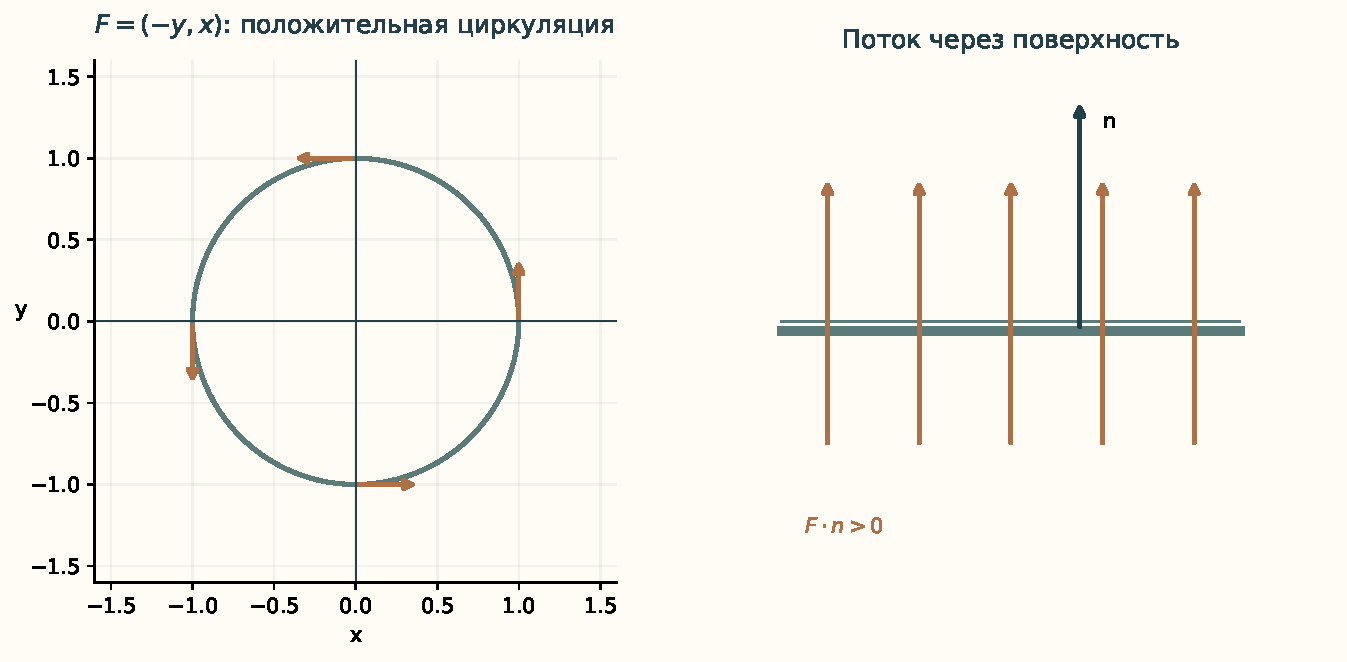
\includegraphics[width=\textwidth,height=.79\textheight,keepaspectratio]{images/atlas-line-surface.pdf}\par\small Направление обхода, нормаль и поток\end{center}\end{minipage}\par
\Needspace{7\baselineskip}\section*{Задачи}
\begingroup\setlength{\parskip}{1pt}
\noindent\begin{minipage}[t]{\linewidth}\textbf{35.1.} Найди массу однородной проволоки единичной линейной плотности на отрезке от \((0,0)\) до \((3,4)\) через интеграл первого рода.\par\end{minipage}\par
\noindent\begin{minipage}[t]{\linewidth}\textbf{35.2.} Вычисли \(\int_\gamma x\,ds\), где \(\gamma(t)=(2t,0)\), \(0\le t\le1\).\par\end{minipage}\par
\noindent\begin{minipage}[t]{\linewidth}\textbf{35.3.} Найди \(\oint_\gamma1\,ds\) по единичной окружности.\par\end{minipage}\par
\noindent\begin{minipage}[t]{\linewidth}\textbf{35.4.} Найди длину одного витка винтовой линии \(\gamma(t)=(\cos t,\sin t,t)\), \(0\le t\le2\pi\).\par\end{minipage}\par
\noindent\begin{minipage}[t]{\linewidth}\textbf{35.5.} Поле \(F=(1,2)\) действует на прямолинейном пути от \((0,0)\) до \((3,4)\). Вычисли работу.\par\end{minipage}\par
\par\addvspace{5pt}\begin{lrbox}{\CatFlowBox}\begin{minipage}[t]{\linewidth}
\setlength{\parskip}{5pt}\setlength{\columnsep}{4.5mm}\setlength{\intextsep}{0pt}
\begin{wrapfigure}[9]{r}{54mm}

\includegraphics[width=54mm,height=58mm,keepaspectratio]{images/unique/art-164.png}
\end{wrapfigure}
\textbf{35.6.} Найди \(\int_\gamma y\,dx+x\,dy\) по любому кусочно гладкому пути от \((0,0)\) до \((1,2)\).\par

\textbf{35.7.} Вычисли циркуляцию \((-y,x)\) по единичной окружности против часовой стрелки.\par

\textbf{35.8.} Как изменятся ответ предыдущей задачи и длина окружности при обходе по часовой стрелке?\par

\textbf{35.9.}\starmark{} Проверь нулевой плоский ротор поля \((-\dfrac y{x^2+y^2},\dfrac x{x^2+y^2})\) вне нуля и вычисли циркуляцию по единичной окружности. Есть ли глобальный потенциал на проколотой плоскости? Обход — против часовой стрелки.\par
\par\WFclear\end{minipage}\end{lrbox}%
\ifdim\dimexpr\ht\CatFlowBox+\dp\CatFlowBox\relax<64mm\dp\CatFlowBox=\dimexpr64mm-\ht\CatFlowBox\relax\fi%
\noindent\usebox{\CatFlowBox}\par\addvspace{5pt}

\noindent\begin{minipage}[t]{\linewidth}\textbf{35.10.} Для \(z(t)=2e^{it}\), \(0\le t\le2\pi\), вычисли \(\oint_\gamma\dfrac1z\,dz\).\par\end{minipage}\par
\noindent\begin{minipage}[t]{\linewidth}\textbf{35.11.} По тому же контуру вычисли \(\oint_\gamma z\,dz\).\par\end{minipage}\par
\noindent\begin{minipage}[t]{\linewidth}\textbf{35.12.} Используя Грина, вычисли \(\oint_{\partial D}x\,dy\) для \(D=[0;2]\times[0;3]\) с положительным обходом.\par\end{minipage}\par
\noindent\begin{minipage}[t]{\linewidth}\textbf{35.13.} Проверь формулу площади \(S=\dfrac12\oint(x\,dy-y\,dx)\) для положительно ориентированного треугольника \((0,0),(2,0),(0,3)\).\par\end{minipage}\par
\noindent\begin{minipage}[t]{\linewidth}\textbf{35.14.} Найди площадь графика \(z=2x\) над единичным квадратом.\par\end{minipage}\par
\noindent\begin{minipage}[t]{\linewidth}\textbf{35.15.} На единичном квадрате в плоскости \(z=0\) поверхностная плотность \(3\). Найди массу.\par\end{minipage}\par
\noindent\begin{minipage}[t]{\linewidth}\textbf{35.16.} Вычисли площадь сферы радиуса \(2\) её параметризацией.\par\end{minipage}\par
\noindent\begin{minipage}[t]{\linewidth}\textbf{35.17.} Найди площадь боковой поверхности цилиндра \(r=2,h=3\) через \(\symbf r(\theta,z)=(2\cos\theta,2\sin\theta,z)\).\par\end{minipage}\par
\noindent\begin{minipage}[t]{\linewidth}\textbf{35.18.} Поле \(F=(0,0,3)\) проходит через круг радиуса \(2\) в плоскости \(z=0\). Найди поток при нормали вверх и вниз.\par\end{minipage}\par
\noindent\begin{minipage}[t]{\linewidth}\textbf{35.19.} Вычисли внешний поток \(F=(x,y,z)\) через сферу радиуса \(2\) непосредственно и через Гаусса.\par\end{minipage}\par
\noindent\begin{minipage}[t]{\linewidth}\textbf{35.20.} Вычисли внешний поток \(F=(x,y,z)\) через границу единичного куба.\par\end{minipage}\par
\noindent\begin{minipage}[t]{\linewidth}\textbf{35.21.} Найди \(\operatorname{div}(x^2,y^2,z^2)\) и \(\operatorname{rot}(-\dfrac y2,\dfrac x2,0)\).\par\end{minipage}\par
\noindent\begin{minipage}[t]{\linewidth}\textbf{35.22.}\starmark{} Проверь Стокса для поля \((-\dfrac y2,\dfrac x2,0)\) и единичного диска \(z=0\) с нормалью вверх.\par\end{minipage}\par
\noindent\begin{minipage}[t]{\linewidth}\textbf{35.23.}\starmark{} Докажи, что при замене \(\widetilde\gamma(t)=\gamma(a+b-t)\) интеграл первого рода сохраняется, а второго меняет знак.\par\end{minipage}\par
\noindent\begin{minipage}[t]{\linewidth}\textbf{35.24.}\starmark{} Докажи, что циркуляция градиента \(C^1\)-функции по любой замкнутой кусочно гладкой кривой в её области определения равна нулю.\par\end{minipage}\par
\endgroup
